\documentclass{standalone}
\usepackage{tikz}
\usetikzlibrary{patterns, positioning}
\usepackage[sfdefault]{ClearSans} %% option 'sfdefault' activates Clear Sans as the default text font
\usepackage[T1]{fontenc}

\begin{document}
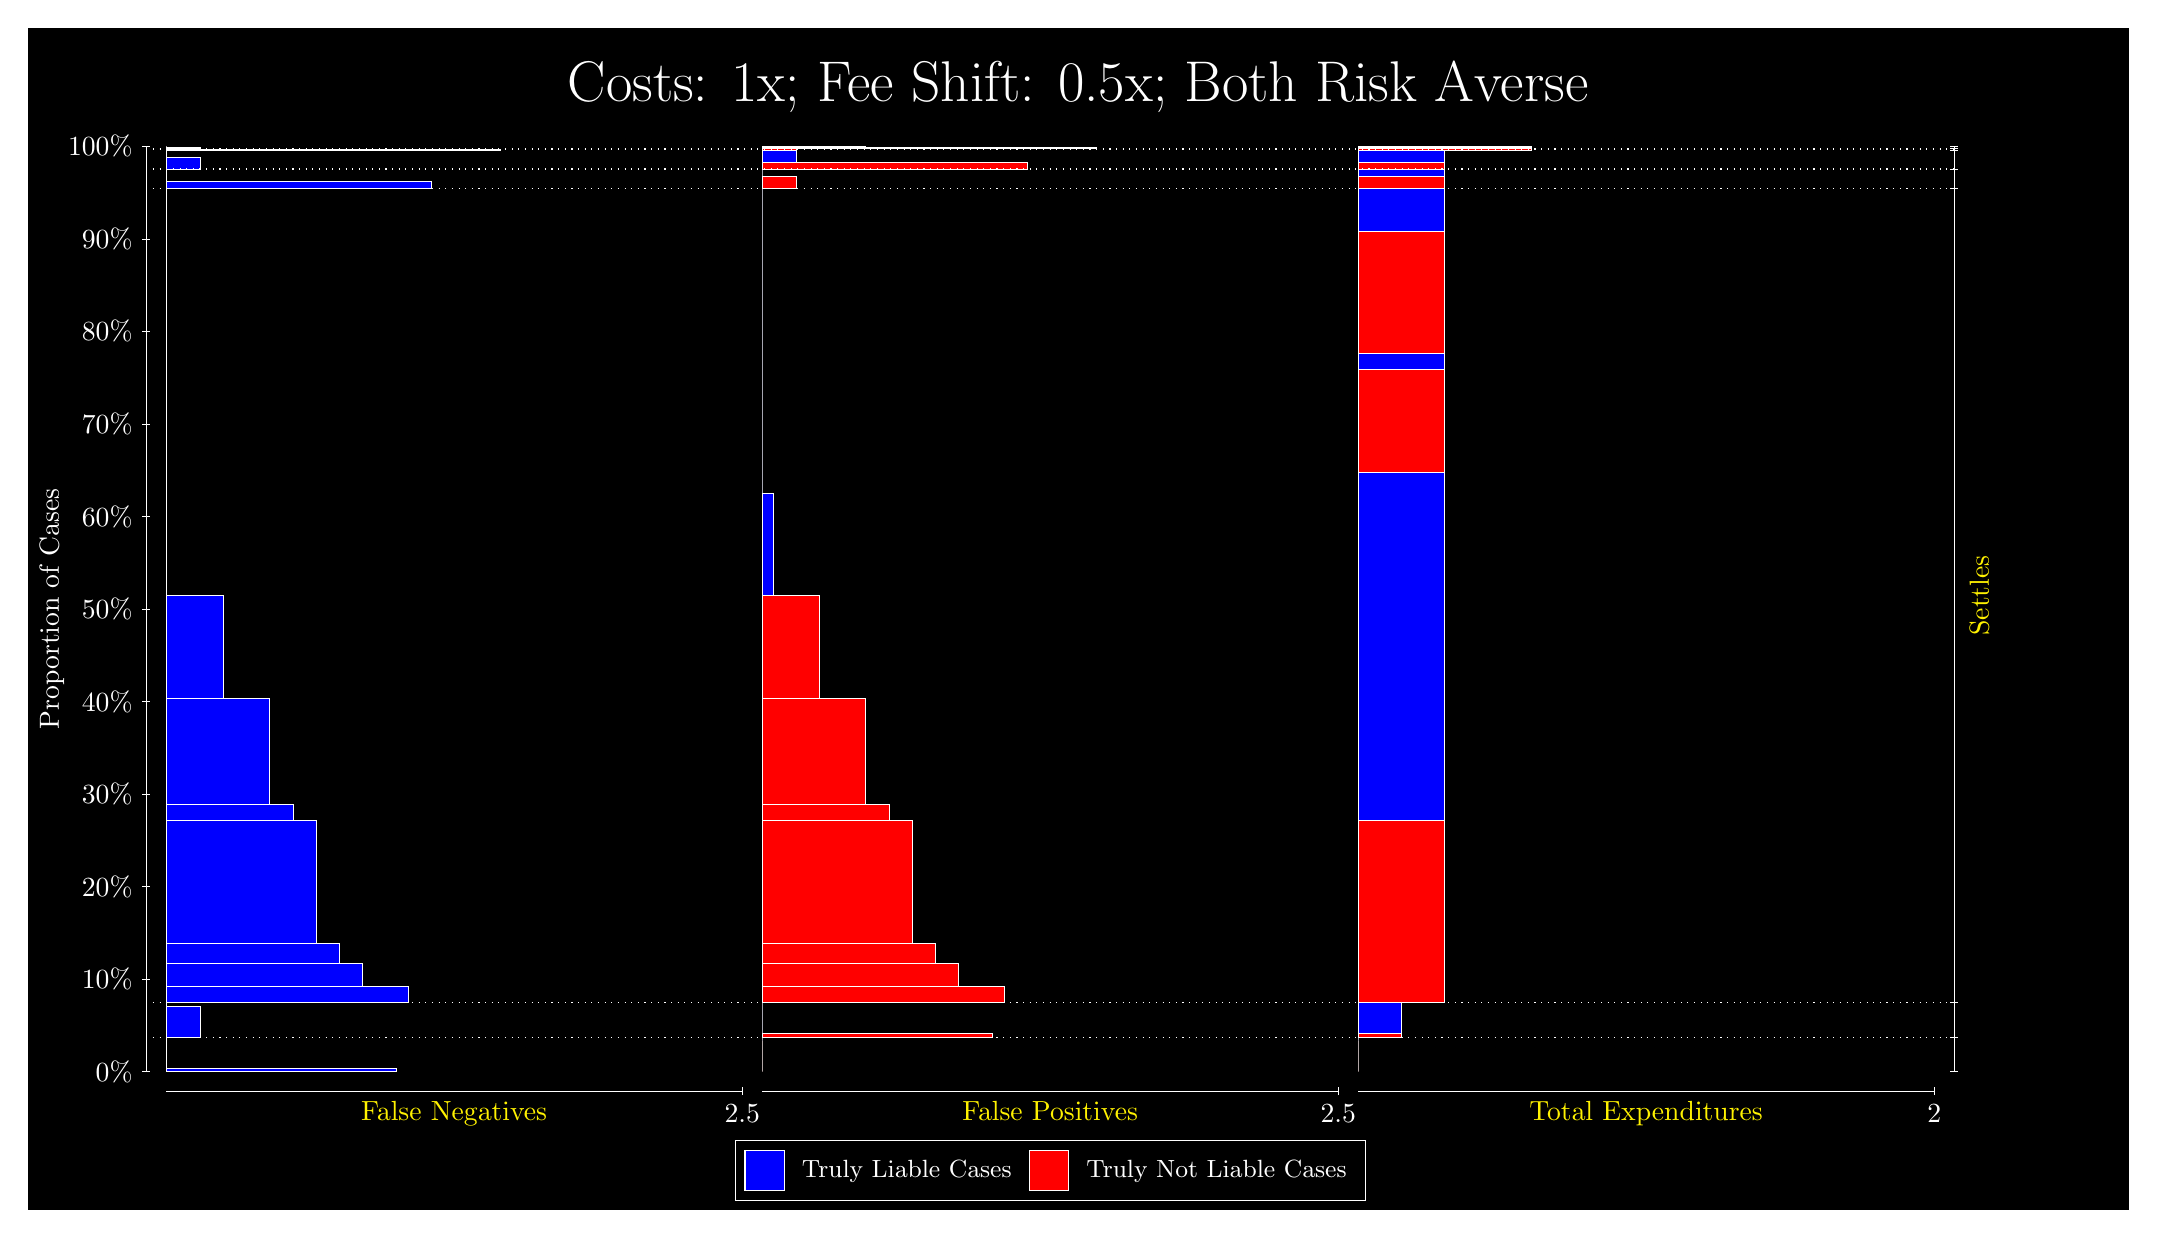
\begin{tikzpicture}
\draw[fill=black] (0,0) rectangle (26.667,15);
\draw[text=white] (0,13.5) rectangle (26.667,15) node[midway] {\huge Costs: 1x; Fee Shift: 0.5x; Both Risk Averse};
\draw[white, very thin] (1.5,1.75) -- (1.5,13.5);
\node[rotate=90, text=white, anchor=center] at (0.3, 7.625) {Proportion of Cases};
\draw[white, very thin] (1.45,1.75) -- (1.55,1.75);
\node[text=white, anchor=east] at (1.45, 1.75) {0\%};
\draw[white, very thin] (1.45,2.925) -- (1.55,2.925);
\node[text=white, anchor=east] at (1.45, 2.925) {10\%};
\draw[white, very thin] (1.45,4.1) -- (1.55,4.1);
\node[text=white, anchor=east] at (1.45, 4.1) {20\%};
\draw[white, very thin] (1.45,5.275) -- (1.55,5.275);
\node[text=white, anchor=east] at (1.45, 5.275) {30\%};
\draw[white, very thin] (1.45,6.45) -- (1.55,6.45);
\node[text=white, anchor=east] at (1.45, 6.45) {40\%};
\draw[white, very thin] (1.45,7.625) -- (1.55,7.625);
\node[text=white, anchor=east] at (1.45, 7.625) {50\%};
\draw[white, very thin] (1.45,8.8) -- (1.55,8.8);
\node[text=white, anchor=east] at (1.45, 8.8) {60\%};
\draw[white, very thin] (1.45,9.975) -- (1.55,9.975);
\node[text=white, anchor=east] at (1.45, 9.975) {70\%};
\draw[white, very thin] (1.45,11.15) -- (1.55,11.15);
\node[text=white, anchor=east] at (1.45, 11.15) {80\%};
\draw[white, very thin] (1.45,12.325) -- (1.55,12.325);
\node[text=white, anchor=east] at (1.45, 12.325) {90\%};
\draw[white, very thin] (1.45,13.5) -- (1.55,13.5);
\node[text=white, anchor=east] at (1.45, 13.5) {100\%};

\draw[white, very thin] (24.457,1.75) -- (24.457,13.5);
\draw[white, very thin] (24.407,1.75) -- (24.507,1.75);
\node[anchor=west] at (24.407, 1.75) {};
\draw[white, very thin] (24.407,2.1873) -- (24.507,2.1873);
\node[anchor=west] at (24.407, 2.1873) {};
\draw[white, very thin] (24.407,2.6245) -- (24.507,2.6245);
\node[anchor=west] at (24.407, 2.6245) {};
\draw[white, very thin] (24.407,12.97) -- (24.507,12.97);
\node[anchor=west] at (24.407, 12.97) {};
\draw[white, very thin] (24.407,13.212) -- (24.507,13.212);
\node[anchor=west] at (24.407, 13.212) {};
\draw[white, very thin] (24.407,13.455) -- (24.507,13.455);
\node[anchor=west] at (24.407, 13.455) {};
\draw[white, very thin] (24.407,13.477) -- (24.507,13.477);
\node[anchor=west] at (24.407, 13.477) {};
\draw[white, very thin] (24.407,13.5) -- (24.507,13.5);
\node[anchor=west] at (24.407, 13.5) {};

\draw[white, very thin, fill=blue] (1.75,1.75) rectangle (4.6775,1.796);
\draw[white, very thin, fill=red] (1.75,1.796) rectangle (1.75,2.1873);
\draw[white, very thin, fill=blue] (1.75,2.1873) rectangle (2.1891,2.5785);
\draw[white, very thin, fill=red] (1.75,2.5785) rectangle (1.75,2.6245);
\draw[white, very thin, fill=blue] (1.75,2.6245) rectangle (4.8239,2.8285);
\draw[white, very thin, fill=blue] (1.75,2.8285) rectangle (4.2384,3.121);
\draw[white, very thin, fill=blue] (1.75,3.121) rectangle (3.9457,3.3751);
\draw[white, very thin, fill=blue] (1.75,3.3751) rectangle (3.6529,4.9443);
\draw[white, very thin, fill=blue] (1.75,4.9443) rectangle (3.3602,5.1446);
\draw[white, very thin, fill=blue] (1.75,5.1446) rectangle (3.0674,6.4943);
\draw[white, very thin, fill=blue] (1.75,6.4943) rectangle (2.4819,7.797);
\draw[white, very thin, fill=red] (1.75,7.797) rectangle (1.75,12.97);
\draw[white, very thin, fill=blue] (1.75,12.97) rectangle (5.1167,13.06);
\draw[white, very thin, fill=red] (1.75,13.06) rectangle (1.75,13.212);
\draw[white, very thin, fill=blue] (1.75,13.212) rectangle (2.1891,13.364);
\draw[white, very thin, fill=red] (1.75,13.364) rectangle (1.75,13.455);
\draw[white, very thin, fill=blue] (1.75,13.455) rectangle (5.9949,13.462);
\draw[white, very thin, fill=red] (1.75,13.462) rectangle (1.75,13.477);
\draw[white, very thin, fill=blue] (1.75,13.477) rectangle (2.1891,13.493);
\draw[white, very thin, fill=red] (1.75,13.493) rectangle (1.75,13.5);
\draw[white, very thin, fill=red] (9.3189,1.75) rectangle (9.3189,2.1413);
\draw[white, very thin, fill=blue] (9.3189,2.1413) rectangle (9.3189,2.1873);
\draw[white, very thin, fill=red] (9.3189,2.1873) rectangle (12.246,2.2333);
\draw[white, very thin, fill=blue] (9.3189,2.2333) rectangle (9.3189,2.6245);
\draw[white, very thin, fill=red] (9.3189,2.6245) rectangle (12.393,2.8285);
\draw[white, very thin, fill=red] (9.3189,2.8285) rectangle (11.807,3.121);
\draw[white, very thin, fill=red] (9.3189,3.121) rectangle (11.515,3.3752);
\draw[white, very thin, fill=red] (9.3189,3.3752) rectangle (11.222,4.9444);
\draw[white, very thin, fill=red] (9.3189,4.9444) rectangle (10.929,5.1447);
\draw[white, very thin, fill=red] (9.3189,5.1447) rectangle (10.636,6.4944);
\draw[white, very thin, fill=red] (9.3189,6.4944) rectangle (10.051,7.7971);
\draw[white, very thin, fill=blue] (9.3189,7.7971) rectangle (9.4652,9.0997);
\draw[white, very thin, fill=blue] (9.3189,9.0997) rectangle (9.3189,12.97);
\draw[white, very thin, fill=red] (9.3189,12.97) rectangle (9.758,13.122);
\draw[white, very thin, fill=blue] (9.3189,13.122) rectangle (9.3189,13.212);
\draw[white, very thin, fill=red] (9.3189,13.212) rectangle (12.686,13.303);
\draw[white, very thin, fill=blue] (9.3189,13.303) rectangle (9.758,13.455);
\draw[white, very thin, fill=red] (9.3189,13.455) rectangle (9.758,13.47);
\draw[white, very thin, fill=blue] (9.3189,13.47) rectangle (9.3189,13.477);
\draw[white, very thin, fill=red] (9.3189,13.477) rectangle (13.564,13.485);
\draw[white, very thin, fill=blue] (9.3189,13.485) rectangle (10.636,13.5);
\draw[white, very thin, fill=red] (16.888,1.75) rectangle (16.888,2.1413);
\draw[white, very thin, fill=blue] (16.888,2.1413) rectangle (16.888,2.1873);
\draw[white, very thin, fill=red] (16.888,2.1873) rectangle (17.437,2.2333);
\draw[white, very thin, fill=blue] (16.888,2.2333) rectangle (17.437,2.6245);
\draw[white, very thin, fill=red] (16.888,2.6245) rectangle (17.986,4.9444);
\draw[white, very thin, fill=blue] (16.888,4.9444) rectangle (17.986,9.3663);
\draw[white, very thin, fill=red] (16.888,9.3663) rectangle (17.986,10.669);
\draw[white, very thin, fill=blue] (16.888,10.669) rectangle (17.986,10.873);
\draw[white, very thin, fill=red] (16.888,10.873) rectangle (17.986,12.423);
\draw[white, very thin, fill=blue] (16.888,12.423) rectangle (17.986,12.97);
\draw[white, very thin, fill=red] (16.888,12.97) rectangle (17.986,13.122);
\draw[white, very thin, fill=blue] (16.888,13.122) rectangle (17.986,13.212);
\draw[white, very thin, fill=red] (16.888,13.212) rectangle (17.986,13.303);
\draw[white, very thin, fill=blue] (16.888,13.303) rectangle (17.986,13.455);
\draw[white, very thin, fill=red] (16.888,13.455) rectangle (19.083,13.47);
\draw[white, very thin, fill=blue] (16.888,13.47) rectangle (19.083,13.477);
\draw[white, very thin, fill=red] (16.888,13.477) rectangle (19.083,13.485);
\draw[white, very thin, fill=blue] (16.888,13.485) rectangle (19.083,13.5);
\draw[white, dotted] (1.5,2.1873) -- (24.457,2.1873);
\draw[white, dotted] (1.5,2.6245) -- (24.457,2.6245);
\draw[white, dotted] (1.5,12.97) -- (24.457,12.97);
\draw[white, dotted] (1.5,13.212) -- (24.457,13.212);
\draw[white, dotted] (1.5,13.455) -- (24.457,13.455);
\draw[white, dotted] (1.5,13.477) -- (24.457,13.477);
\draw[white, very thin] (1.75,1.5) -- (9.0689,1.5);
\node[text=yellow, anchor=north] at (5.4094, 1.5) {False Negatives};
\draw[white, very thin] (9.0689,1.45) -- (9.0689,1.55);
\node[text=white, anchor=north] at (9.0689, 1.45) {2.5};

\draw[white, very thin] (9.3189,1.5) -- (16.638,1.5);
\node[text=yellow, anchor=north] at (12.978, 1.5) {False Positives};
\draw[white, very thin] (16.638,1.45) -- (16.638,1.55);
\node[text=white, anchor=north] at (16.638, 1.45) {2.5};

\draw[white, very thin] (16.888,1.5) -- (24.207,1.5);
\node[text=yellow, anchor=north] at (20.547, 1.5) {Total Expenditures};
\draw[white, very thin] (24.207,1.45) -- (24.207,1.55);
\node[text=white, anchor=north] at (24.207, 1.45) {2};



\node[text=yellow, centered, rotate=90] at (24.777, 7.797) {Settles};





\draw (12.978300999999998,1.5) node[draw=none] (baseCoordinate) {};
\begin{scope}[align=center]
        \matrix[scale=0.5, draw=white, below=0.5cm of baseCoordinate, nodes={draw}, column sep=0.1cm]{
            \node[rectangle, draw, minimum width=0.5cm, minimum height=0.5cm, fill=blue] {}; &
            \node[draw=none, font=\small, text=white] (B) {Truly Liable Cases}; &
            \node[rectangle, draw, minimum width=0.5cm, minimum height=0.5cm, fill=red] {}; &
            \node[draw=none, font=\small, text=white] (B) {Truly Not Liable Cases}; \\
            };
\end{scope}

\end{tikzpicture}
\end{document}